\citeonline{Botsal1999} exemplifica o \textit{lot streaming} apresentando um modelo básico que dá a ideia de como a técnica é capaz de acelerar o processo e, por consequência, diminuir o \textit{makespan}. No exemplo, mostrado na Figura~\ref{fig:LSBasic}, há um lote de 500 unidades sendo processado em um sistema de 2 máquinas com tempos de processamento distintos ($p_1=2$ unidades de tempo para a máquina M1, e $p_2=1$ unidade de tempo para a máquina M2). De acordo com o processo de manufatura tradicional, o \textit{makespan} total é de 1.500 unidades de tempo para processar as 500 unidades, sendo $500 \times 2 + 500 \times 1 = 1.500$. Considerando então a divisão em dois sublotes de tamanhos 300 e 200 unidades, o \textit{makespan} passa a ser, agora, no tempo total de 1.200 unidades de tempo.

\begin{figure}[!ht]
    \begin{center}
    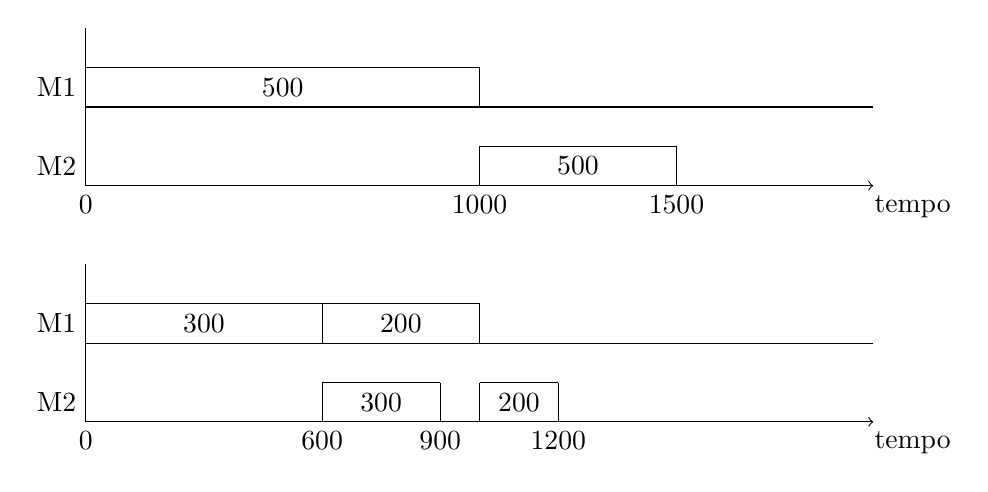
\begin{tikzpicture}
    %% X
    \draw[->] (0,0) -- (10,0); \draw (10.5,0) node[below] {tempo}; \draw (6.25,0.25) node {500}; \draw (5,0) node[below] {1000}; \draw (7.5,0) node[below] {1500};
    %% Y
    \draw[-] (0,0) -- (0,2); \draw (0,0) node[below] {0};
    %% M1
    \draw[-] (0,1.5) -- (5,1.5); \draw[-] (5,1.5) -- (5,1); \draw (2.5,1.25) node {500}; \draw (0,1.25) node[left] {M1};
    %% MEIO
    \draw[-] (0,1) -- (10,1);
    %% M2
    \draw[-] (5,0) -- (5,0.5); \draw[-] (5,0.5) -- (7.5,0.5); \draw[-] (7.5,0.5) -- (7.5,0); \draw (0,0.25) node[left] {M2};
    %% GRAFO DE BAIXO
    %% X
    \draw[->](0,-3)--(10,-3); \draw (10.5,-3) node[below] {tempo}; \draw(3,-3) node[below]{600}; \draw(4.5,-3) node[below]{900}; \draw(6,-3) node[below]{1200};
    %% Y
    \draw[-](0,-1) -- (0,-3); \draw (0,-2.75) node[left] {M2}; \draw (0,-3) node[below] {0};
    %% M1
    \draw[-] (0,-1.5) -- (5,-1.5); \draw[-] (5,-1.5)--(5,-2); \draw[-] (3,-1.5)--(3,-2); \draw (1.5,-1.75) node{300}; \draw (4,-1.75) node{200}; \draw (0,-1.75) node[left] {M1};
    %% MEIO
    \draw[-] (0,-2) -- (10,-2);
    %% M2
    \draw[-](3,-3) -- (3,-2.5); \draw[-] (3,-2.5) -- (4.5,-2.5); \draw[-] (4.5,-2.5) -- (4.5,-3); \draw (3.75,-2.75) node{300}; \draw[-](5,-3) -- (5,-2.5); \draw[-] (5,-2.5) -- (6,-2.5); \draw[-] (6,-2.5) -- (6,-3); \draw (5.5,-2.75) node{200};
    \end{tikzpicture}
    \end{center}
    \caption{Exemplo básico de \citeonline{Botsal1999}.}
    \label{fig:LSBasic}
\end{figure}